\newsection{Anhang}{appendix}

\noindent\textbf{A.1:}\label{app:1}
\begin{equation}\tag{A.1}\label{eq:complex-numbers-multiplication}
  \begin{split}
    (a + bi) \cdot (c + di) \\
    =  c(a + bi) + di(a + bi) \\
    = ac +bci + adi + bdi^2 \\
    = ac + bci + adi \textbf{ - } bd \\
    = ac - bd +(bc + ad)i
  \end{split}
\end{equation}

\noindent\textbf{A.2:}\label{app:2}
\begin{equation}\tag{A.2}\label{eq:complex-numbes-squaring}
  \begin{split}
    z_1^2
    = z_1 \cdot z_1 \\
    = (a + bi) \cdot (a + bi) \\
    = a \cdot (a + bi) + bi \cdot (a + bi) \\
    = a^2 + abi + abi - b^2 \\
    = a^2 - b^2 + 2abi
  \end{split}
\end{equation}

\noindent\textbf{A.3:}\label{app:3}
\begin{figure}[H]\label{fig:benoit-mandelbrot-picture}
\begin{center}
  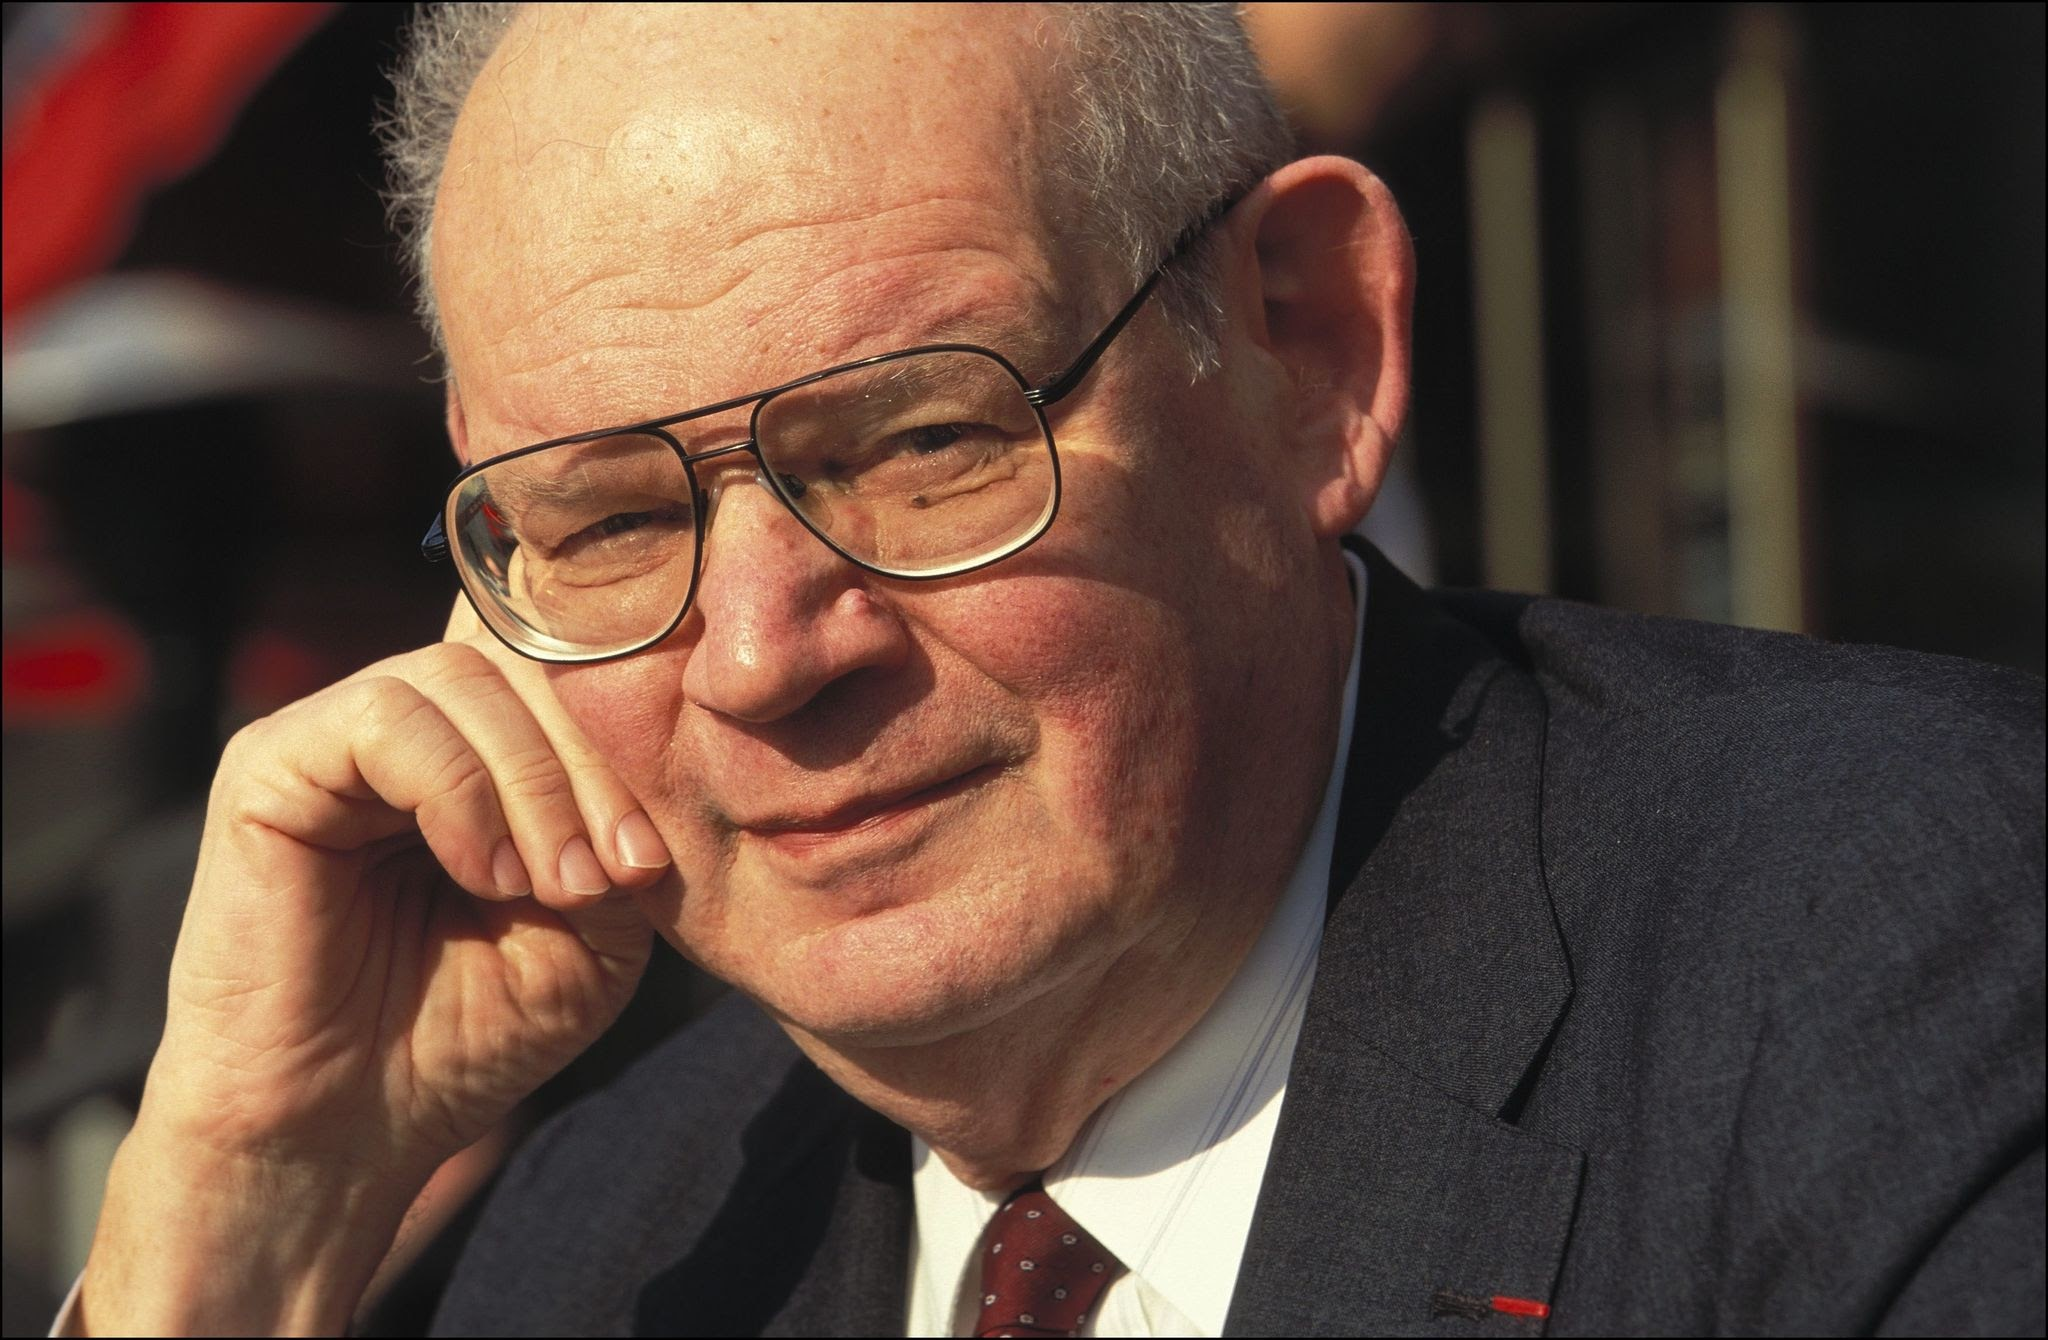
\includegraphics[width=\textwidth]{images/benoit-mandelbrot}
  \caption{Benoît Mandelbrot 1997 in Frankreich~\cite{gaillarde_benoit_1997}}
\end{center}
\end{figure}